\newpage
\subsection*{Karnaugh's maps for Task 3}
For the Moore's state machine implementation:


\begin{figure}[H]
    \begin{center}
         \begin{KarnaughvuitV3}
            \minterms{5,6}
             \maxterms{0,1,2,4}
             \indeterminats{3,7}
            \implicant{7}{6}{red}
            \implicant{5}{7}{green}
         \end{KarnaughvuitV3}
         \begin{KarnaughvuitV3}
            \minterms{2,4,7}
            \maxterms{0,1,3,5,6}
            \implicantsol{2}{red}
            \implicantsol{4}{green}
            \implicantsol{7}{blue}
         \end{KarnaughvuitV3}
         \caption{Maps for $Y_2$ (left) and $Y_1$ (right) functions.}
    \end{center}
    \end{figure}
Where $Y_2 = W \cdot y_1 + W \cdot y_2$, and $Y_1 = W \cdot \overline{y_2} \cdot \overline{y_1}$. 
From the transitions table, it is simple to see that $Z = y_1$.

And for the Mealy's state machine implementation:

\begin{figure}[H]
    \begin{center}
     \begin{KarnaughquatreV3}
         \minterms{1,3}
        \maxterms{0,2}
        \implicant{1}{3}{red}
     \end{KarnaughquatreV3}
     \begin{KarnaughquatreV3}
        \minterms{1}
       \maxterms{0,2,3}
       \implicantsol{1}{red}
    \end{KarnaughquatreV3}
     \caption{Maps for $Y$ (left) and $Z$ (right)}
    \end{center}
\end{figure}
Where from the left map $Y = W$, and from the right
table $Z = \overline{y} \cdot W$.


\subsection*{Level shifter for inputs}
From the implemented circuit:
\begin{figure}[H]
    \begin{centering}
    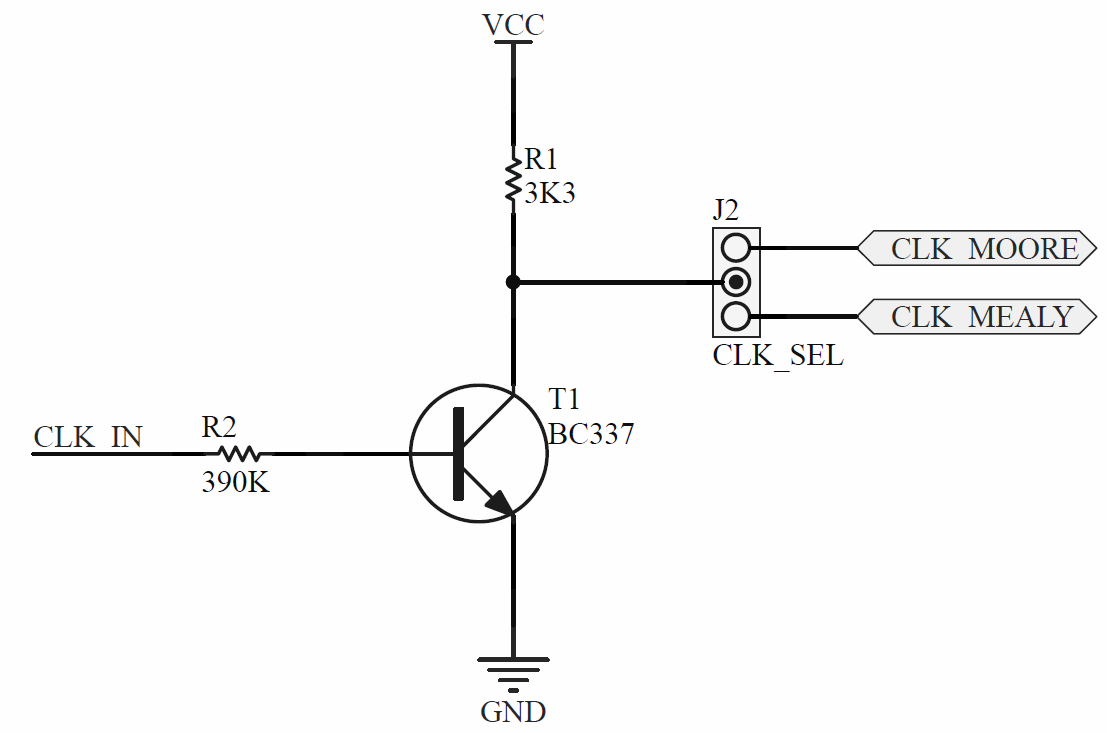
\includegraphics[width=0.5\textwidth]{data/Graficos3/CLK_Driver.png}
    \par\end{centering}
    \caption{Level shifter for CLK from 5V to 3.3V (VCC)}
\end{figure}

Usign for $I_{SAT} = 1mA$, considerating $VCE_{SAT} = 0.2V$, 
the equation from the out mesh:

$$3.3V - VCE_{SAT} - I_{SAT}R_1 = 0$$
$$\frac{3.3V - VCE_{SAT}}{I_{SAT}} = R_1 = 3.1K\Omega$$
Normalizing we have $R_1 = 3.3K\Omega$.
Considering $HFE_{MIN} = 100$, from the input mesh:

$$5V - VBE_{ON} - \frac{I_C}{HFE_{MIN}}R_2 = 0$$
$$\frac{5V - VBE_{ON}}{I_C}HFE_{MIN} = R_2 = 430K\Omega$$
Normalizing we have $R_2 = 390K\Omega$. The same circuit is 
for adapting W input.
\subsection*{Driver for output led}
Taking the implemented circuit:

\begin{figure}[H]
    \begin{centering}
    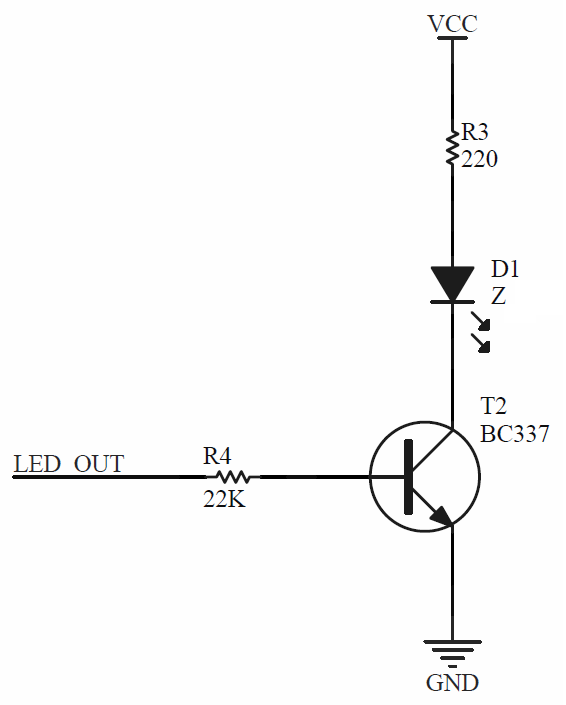
\includegraphics[width=0.4\textwidth]{data/Graficos3/LED_Driver.png}
    \par\end{centering}
    \caption{Driver for LED output.}
\end{figure}

Usign for $I_{LED} = 10mA$, considerating $VCE_{SAT} = 0.2V$ 
and $V{LED} = 2V$, the equation from the out mesh:

$$3.3V - V_{LED} - VCE_{SAT} - I_{LED}R_3 = 0$$
$$\frac{3.3V - V_{LED} - VCE_{SAT}}{I_{LED}} = R_3 = 110\Omega$$
Normalizing we have $R_3 = 220\Omega$.
Considering $HFE_{MIN} = 100$, from the input mesh:

$$3.3V - VBE_{ON} - \frac{I_C}{HFE_{MIN}}R_4 = 0$$
$$\frac{3.3V - VBE_{ON}}{I_C}HFE_{MIN} = R_4 = 26K\Omega$$
Normalizing we have $R_4 = 22K\Omega$, to guarantee saturation.

